\documentclass{article}
\usepackage[utf8]{inputenc}
\usepackage[margin = 0.8in]{geometry}
\usepackage{graphicx}
\usepackage{amsmath, amssymb}
\usepackage{subcaption}
\usepackage{multirow}
\usepackage{mathtools}
\usepackage{float}


\title{RBE502 - Homework Set 6}
\author{Keith Chester}
\date{Due date: October 6 2021}

\begin{document}
\maketitle

\section*{Introduction}

In this assignment, we will be looking at a generic observer-state feedback control system. In this system, we do not have access to the real state when designing a control system and must react to the output of the system. This can occur when sensors do not exist or some other limitation is present to prevent directly observing the current state of the system. A control diagram for this system can be seen below:

\begin{figure}[H]
    \centering
    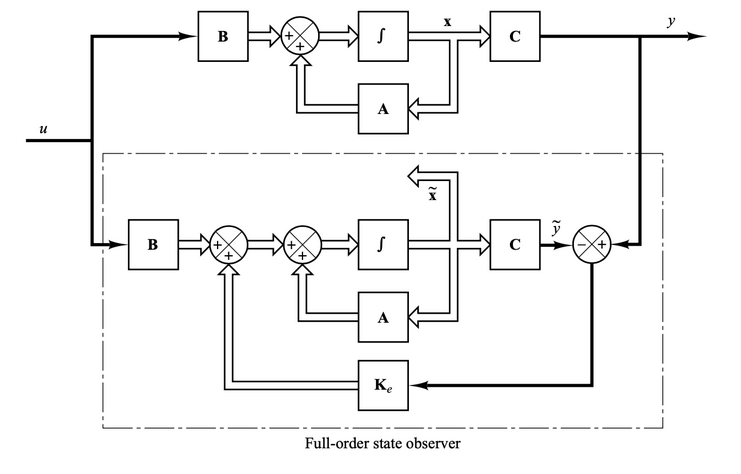
\includegraphics[width = 0.4\textwidth]{figures/system_diagram.png}
    \caption{System diagram of a full order state observer}
    \label{fig:system-diagram}
\end{figure}

Here we consider the system with the standard system equations of:
\begin{equation}
    \dot{x} = \boldsymbol{A}x + \boldsymbol{B}u
\end{equation}
\begin{equation}
    y=\boldsymbol{C}x
\end{equation}

We are given that:

\begin{equation}
    A = \begin{bmatrix}
        0 & 20 \\ 1 & 0 
    \end{bmatrix}
\end{equation}
\begin{equation}
    B = \begin{bmatrix}
        0 \\ 1
    \end{bmatrix}
\end{equation}
\begin{equation}
    C = \begin{bmatrix}
        0 & 1
    \end{bmatrix}
\end{equation}

We aim to, within this homework, design full feedback control $u=-\boldsymbol{K}x$ with desired eigenvalues of a closed loop system $\dot{x}=(\boldsymbol{A}-\boldsymbol{B}\boldsymbol{K})x$ with eigenvalues of $\lambda_1 = -2+5i$ and $\lambda_2= -2-5i$, while only having access to observe the output $y(t)$.

\section*{Part A - Observer Design}
The dynamics of our observer is expressed as:

\begin{equation}
    \dot{\tilde{x}} = (\boldsymbol{A}-\boldsymbol{K}_e \boldsymbol{C})\tilde{x}+\boldsymbol{B}u+K_e y
\end{equation}

We wish to find a suitable $\boldsymbol{K}_e$ such that $\lim_{t \to \infty} ||x-\tilde{x}||=0$.

If we take the original $\dot{x}$ equation earlier and introduce it to our $\dot{\tilde{x}}$ equation, we can then form:

\begin{equation}
    \dot{x}-\dot{\tilde{x}} = (\boldsymbol{A}-\boldsymbol{K}_e\boldsymbol{C})(x-\tilde{x})
\end{equation}

This simplifies the problem to finding a gain matrix $\boldsymbol{K}_e$ such that the eigenvalues of $()\boldsymbol{A}-\boldsymbol{K}_e\boldsymbol{C})$ are have negative real parts. We also know that due to the principle of duality: system 1: $\dot{x} = \boldsymbol{A}x + \boldsymbol{B}u $ and $y=\boldsymbol{C}x$ are equivalent to the dual system, system 2: $\dot{z}=\boldsymbol{A}^T z + \boldsymbol{C}^T v$ and $w = \boldsymbol{B}^T z$. This dual system is formulated as:

\begin{equation}
    \dot{z}=\boldsymbol{A}^T z + \boldsymbol{C}^T v = \begin{bmatrix}
        0 & 1 \\ 20 & 0
    \end{bmatrix} z + \begin{bmatrix}
        0 \\ 1
    \end{bmatrix} v
\end{equation}
\begin{equation}
    w = \boldsymbol{B}^T z = \begin{bmatrix}
        0 & 1
    \end{bmatrix} z
\end{equation}

We can show that our system 1 is observable if the dual system 2 is controllable. To perform a controllability check, we need to see that the resulting rank of what would be the system 2's $\boldsymbol{C}_{ctrl}$ matrix would need to be equivalent to the number of eigenvalues/poles selected - $2$.

\begin{equation}
    rank(\boldsymbol{C}_{ctrl}) = rank(\begin{bmatrix}
        \boldsymbol{A}^0\boldsymbol{B} & \boldsymbol{A}^1\boldsymbol{B}
    \end{bmatrix}) = 2
\end{equation}

\noindent ...however, the resulting values replaced with the transposed matricies from our original system 1:

\begin{equation}
    rank(\boldsymbol{C}_{ctrl}) = rank(\begin{bmatrix}
        (\boldsymbol{A}^T)^0\boldsymbol{C}^T & (\boldsymbol{A}^T)^1\boldsymbol{C}^T
    \end{bmatrix}) = 2
\end{equation}

So, with this formulation in hand, we calculate:

\begin{equation}
    rank(\boldsymbol{C}_{ctrl}) = rank(\begin{bmatrix}
        (\boldsymbol{A}^T)^0\boldsymbol{C}^T & (\boldsymbol{A}^T)^1\boldsymbol{C}^T
    \end{bmatrix}) = rank(\begin{bmatrix}
        \begin{matrix}
            0 \\ 1
        \end{matrix} &
        \begin{matrix}
            1 \\ 0
        \end{matrix}
    \end{bmatrix}) = 2
\end{equation}

Since the rank of our controllability matrix of the dual system 2 is equal to our $n$ of $2$, this confirms that the dual system 2 is controllable. Since our dual system is controllable, our considered system 1 is observable.

Now that we have confirmed this, we wish to utilize Ackermann's formula to find the gain matrix $K_e^T$ that places closed loop eigenvalues of the dual system $\dot{z}=(\boldsymbol{A}^T-\boldsymbol{C}^T\boldsymbol{K}_e^T)z$ at $\mu_1=\mu_2=-10$.

For this, we will first determine the characteristic equation of our chosen eigenvalues $\mu_1$ and $\mu_2$:

\begin{equation}
    \sigma(\boldsymbol{A}^T) = (\lambda-\mu_1)(\lambda-\mu_2) = (\lambda+10)(\lambda+10) = \lambda^2 + 20 \lambda + 100
\end{equation}

With this characteristic equation and the $\boldsymbol{C}_{ctrl}$, we can solve for $\boldsymbol{K}_e^T$ by using a $K_{selector}=\begin{bmatrix}
    0 & 1
\end{bmatrix}$ and $\boldsymbol{A}^T$.

\begin{equation}
    \boldsymbol{K}_e^T = \begin{bmatrix}k_1 & k_2\end{bmatrix} = \boldsymbol{K}_{selector} \boldsymbol{C}_{ctrl}^{-1} \Delta_{new}(\boldsymbol{A}^T)
\end{equation}
\begin{equation}
    \Delta_{new}(\boldsymbol{A}^T) = (\boldsymbol{A}^T)^2+20(\boldsymbol{A}^T)+200\boldsymbol{I}_2 = \begin{bmatrix}
        120 & 20 \\ 400 & 120
    \end{bmatrix}
\end{equation}
\begin{equation}
    \boldsymbol{K}_e^T = \begin{bmatrix}
        0 & 1
    \end{bmatrix} \begin{bmatrix}
        0 & 1 \\ 1 & 0
    \end{bmatrix} \begin{bmatrix}
        120 & 20 \\ 400 & 120
    \end{bmatrix} = \begin{bmatrix}
        120 & 20
    \end{bmatrix}
\end{equation}

Utilizing Ackermann's formula we have found that $\boldsymbol{K}_e^T = \begin{bmatrix}120 & 20\end{bmatrix}$.

\section*{Part B - Controller Design}

Let us now focus on our original main system, 1, or $\dot{x}=\boldsymbol{A}x+\boldsymbol{B}u$ and $y=\boldsymbol{C}x$, is controllable. To do this, we can use the controllability matrix $\boldsymbol{C}_{ctrl}$, where:

\begin{equation}
    rank(\boldsymbol{C}_{ctrl}) = rank(\begin{bmatrix}
        \boldsymbol{A}^0\boldsymbol{B} & \boldsymbol{A}^1\boldsymbol{B}
    \end{bmatrix}) = rank(\begin{bmatrix}
        \begin{matrix}
            0 \\ 1
        \end{matrix} &
        \begin{matrix}
            20 \\ 0
        \end{matrix}
    \end{bmatrix}) = 2
\end{equation}

Since $\boldsymbol{C}_{ctrl}$ has a rank of equal to the number of eigenvalues $count(\lambda)=rank(\boldsymbol{C}_{ctrl})=2$, the system is confirmed to be controllable.

From here we wish to use Ackermann's formula to find a gain matrix $\boldsymbol{K}$ such that the main eigenvalues of the system $\dot{x}=(\boldsymbol{A}-\boldsymbol{B}\boldsymbol{K})$ are $\lambda_1 = -2+5i$ and $\lambda_2 = -2-5i$. First we find the characteristic equation from these eigenvalues, then we use Ackermann's formula to calculate our $\boldsymbol{K}$ using a $\boldsymbol{K}_{selector}=\begin{bmatrix}0 & 1\end{bmatrix}$, the coeffeicients of our characteristic equation, $\boldsymbol{C}_{ctrl}$, and $\Delta_{new}(\boldsymbol{A})$.


\begin{equation}
    (\lambda+2+5i)(\lambda+2-5i) = \lambda^2 + 4\lambda+29
\end{equation}
\begin{equation}
    \boldsymbol{K} = \begin{bmatrix}k_1 & k_2 \end{bmatrix} = \boldsymbol{K}_{selector} \boldsymbol{C}_{ctrl}^{-1} \Delta_{new}(\boldsymbol{A})
\end{equation}
\begin{equation}
    \Delta_{new} = \lambda^2 + 4\lambda+29\boldsymbol{I}_2
\end{equation}
\begin{equation}
    \Delta_{new}(\boldsymbol{A}) = \boldsymbol{A}^2+4\boldsymbol{A}+29\boldsymbol{I}_2
\end{equation}
\begin{equation}
    \boldsymbol{K} = \begin{bmatrix}0 & 1\end{bmatrix} \boldsymbol{C}_{ctrl}^{-1} \Delta_{new}(A) = \begin{bmatrix}
        2.45 & 4
    \end{bmatrix}
\end{equation}

\section*{Part C - Observed-State Feedback Control System}

In part C, we will simulating the observer-state feedback control system and comparing various configuration options throughout. Within this section, we will be assuming the initial conditions of $x_0 = \begin{bmatrix}-1 & 0\end{bmatrix}^T$ and $\tilde{x}_0 = \begin{bmatrix}0 & 1\end{bmatrix}^T$.

\subsection*{Part 1}

In this section, we are looking at the controller $u=-\boldsymbol{K}x$. We simulate our system and produce the following plots of the system's response:

\begin{figure}[H]
    \centering
    \begin{subfigure}{0.325\textwidth}
        \centering
        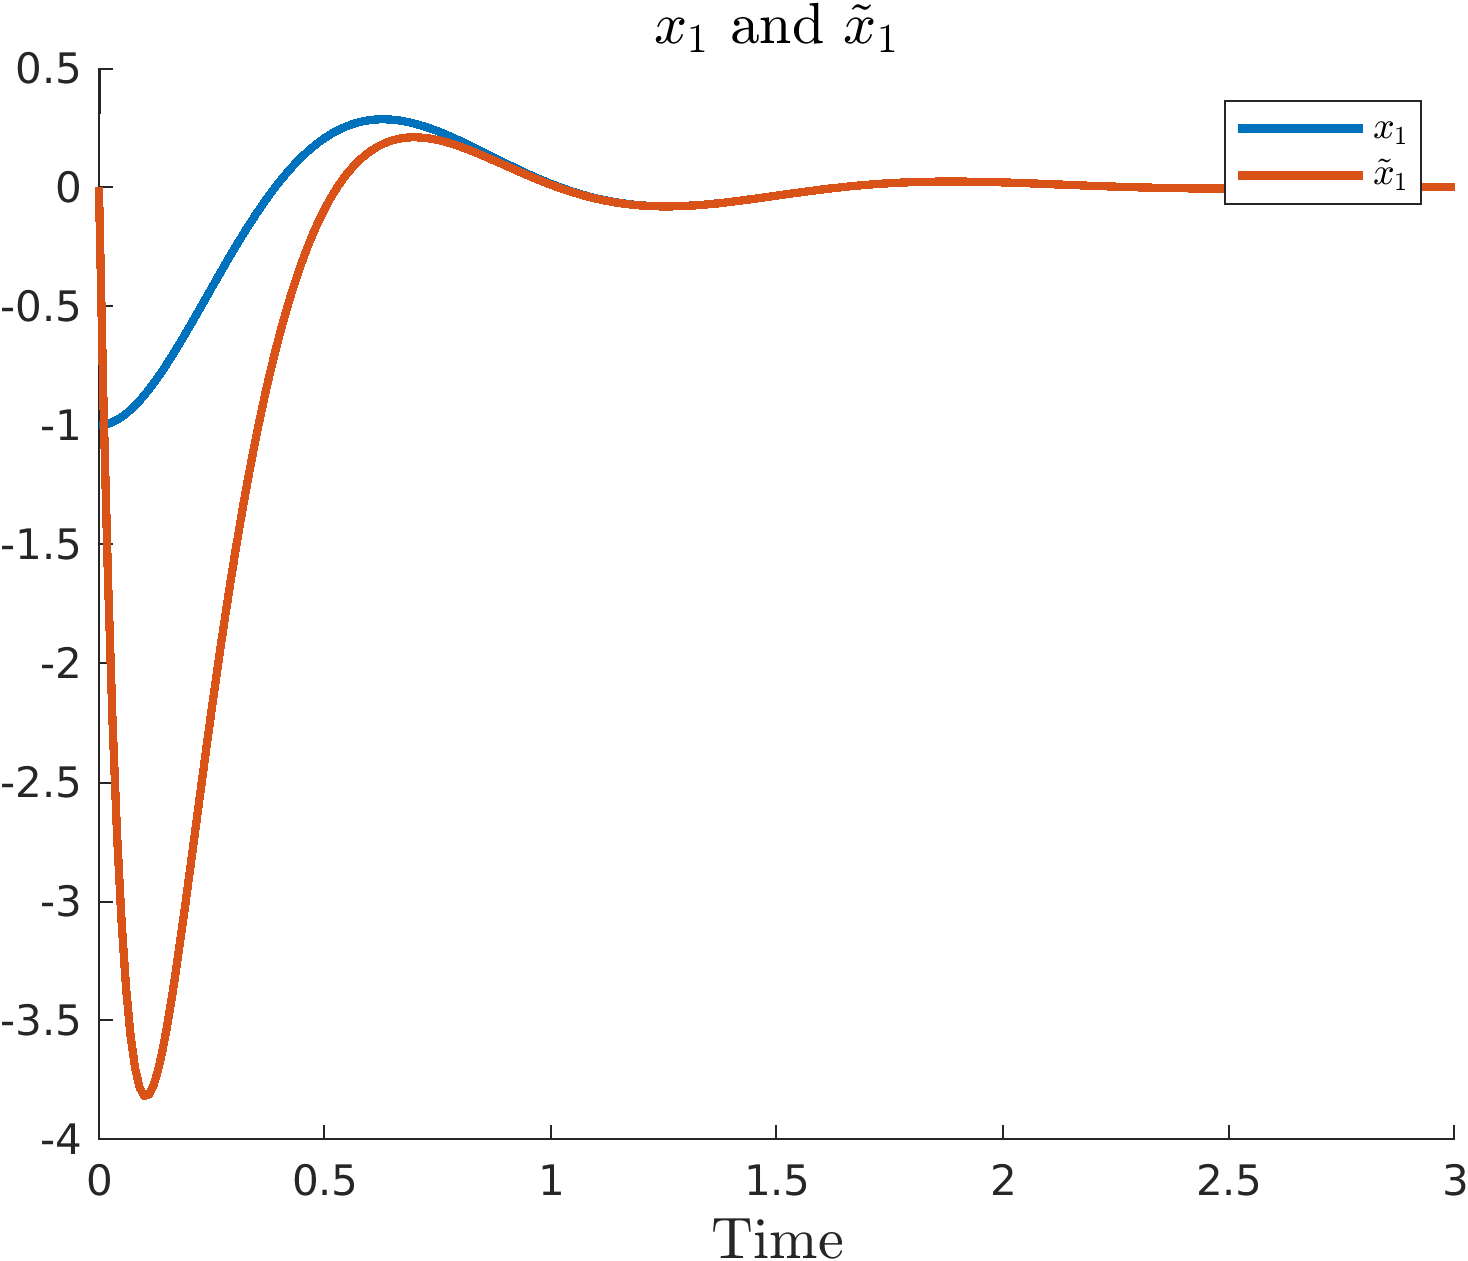
\includegraphics[width = \textwidth]{figures/c1-x1-plot.png}
        \caption{$x_1$ and $\tilde{x}_1$}
    \end{subfigure}
    \begin{subfigure}{0.325\textwidth}
        \centering
        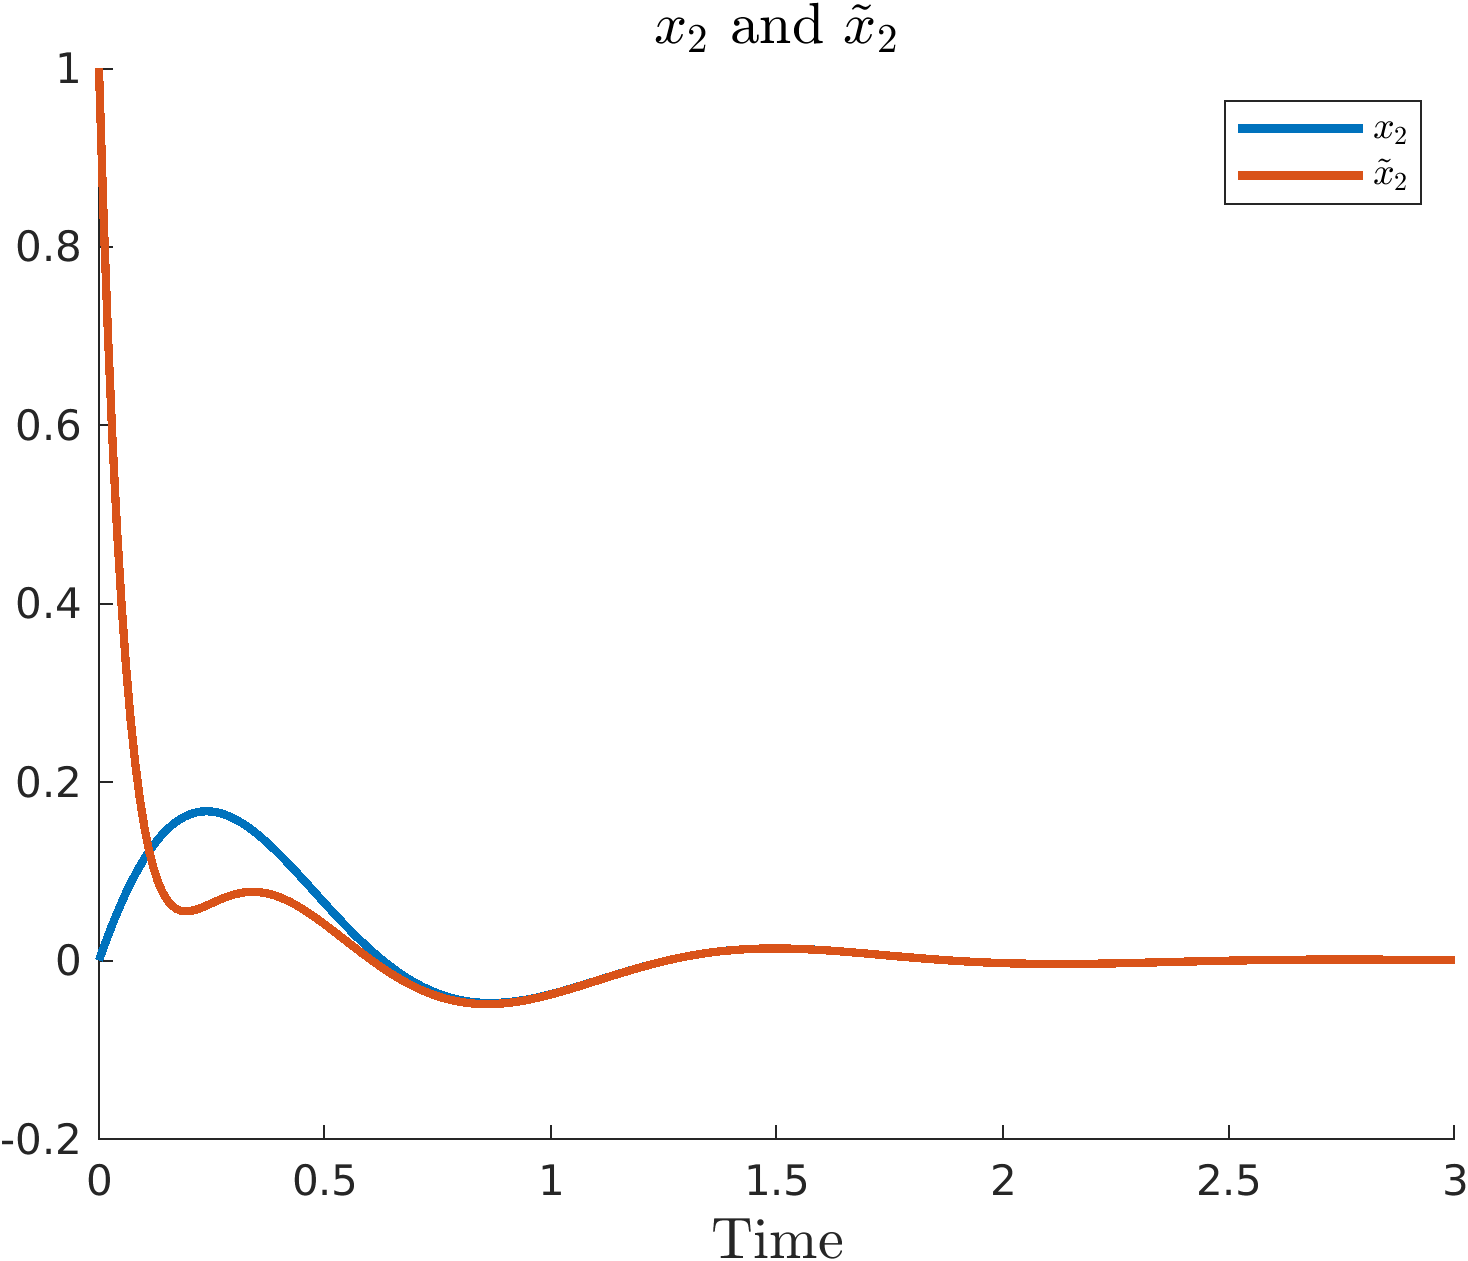
\includegraphics[width = \textwidth]{figures/c1-x2-plot.png}
        \caption{$x_2$ and $\tilde{x}_2$}
    \end{subfigure}
    \caption{Observed-state feedback control system with $u = -\boldsymbol{K}x$}
    \label{fig:c-1_results}
\end{figure}

Here we see that the $\tilde{x}$ response starts out significantly off from the real system state of $x$. Within a half second, both the $x$ and $\tilde{x}$ converge and is in near lockstep from there on out. The system quickly stabilizes within approximately $2$ seconds.

\subsection*{Part 2}

In this part, we will be exploring the system with $u=-\boldsymbol{K}\tilde{x}$ versus the previously utilized $u=-\boldsymbol{K}\tilde{x}$. Below we see the real $x$ response of our system:

\begin{figure}[H]
    \centering
    \begin{subfigure}{0.325\textwidth}
        \centering
        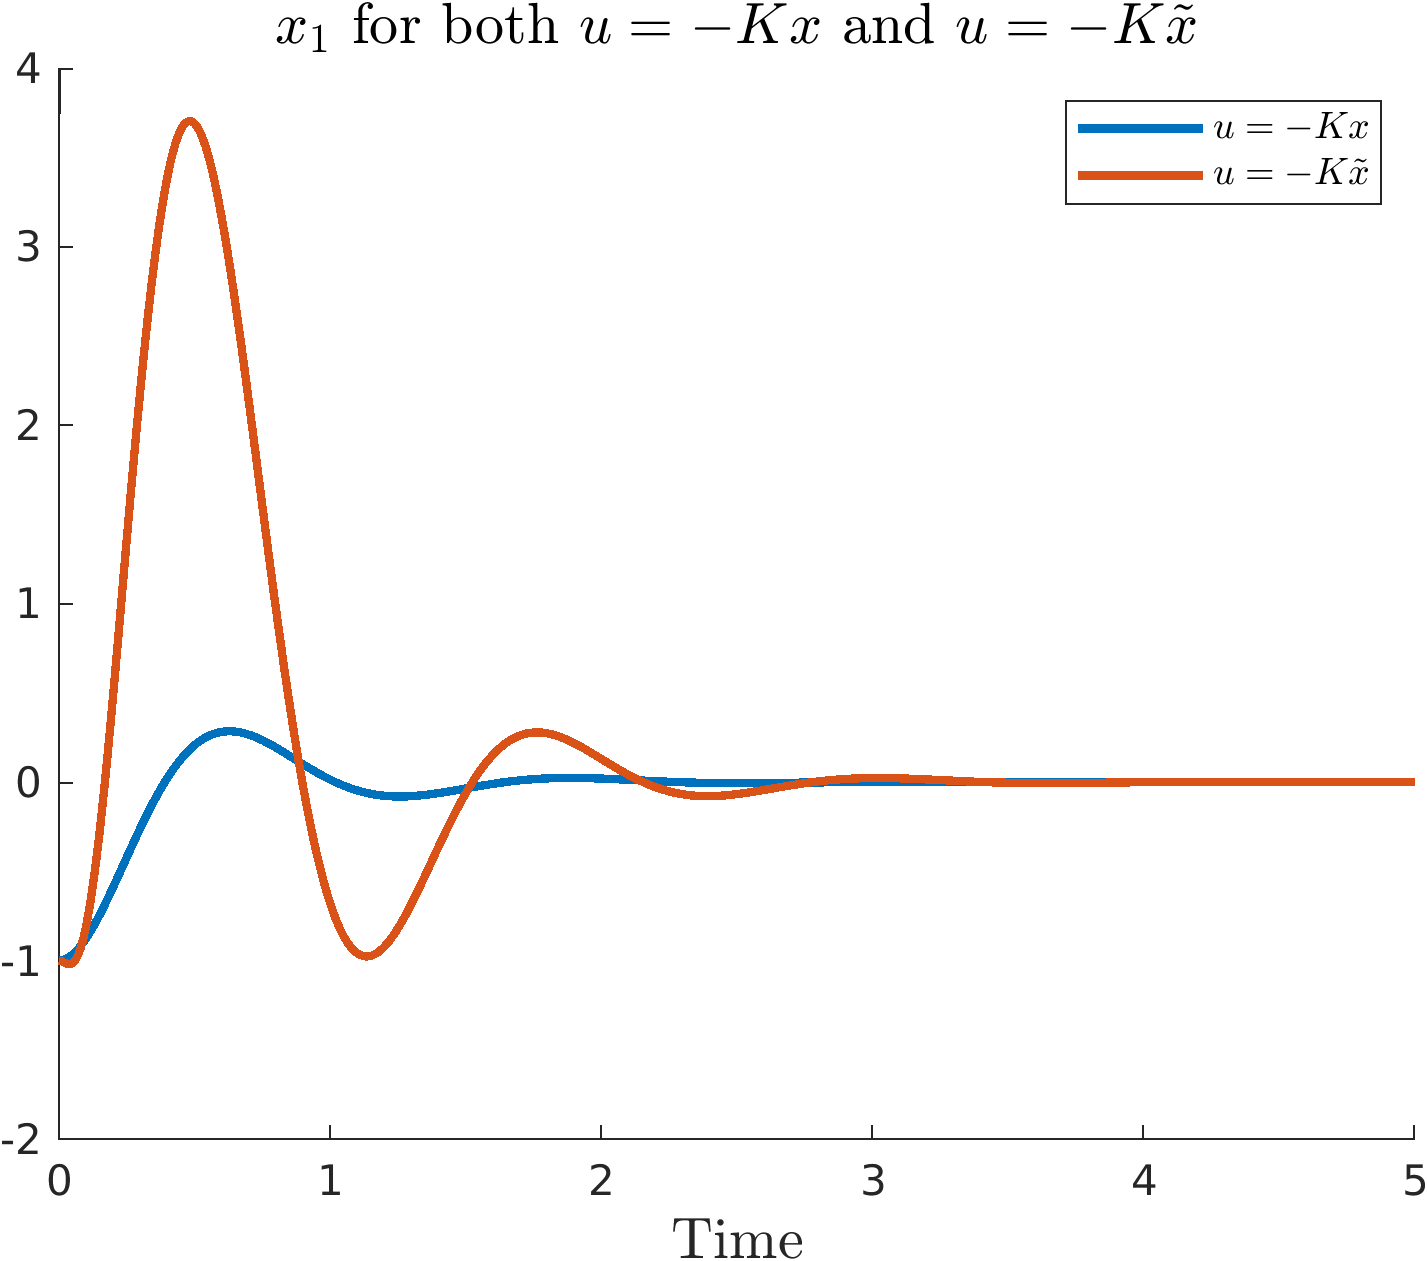
\includegraphics[width = \textwidth]{figures/c2-x1-plot.png}
    \end{subfigure}
    \begin{subfigure}{0.325\textwidth}
        \centering
        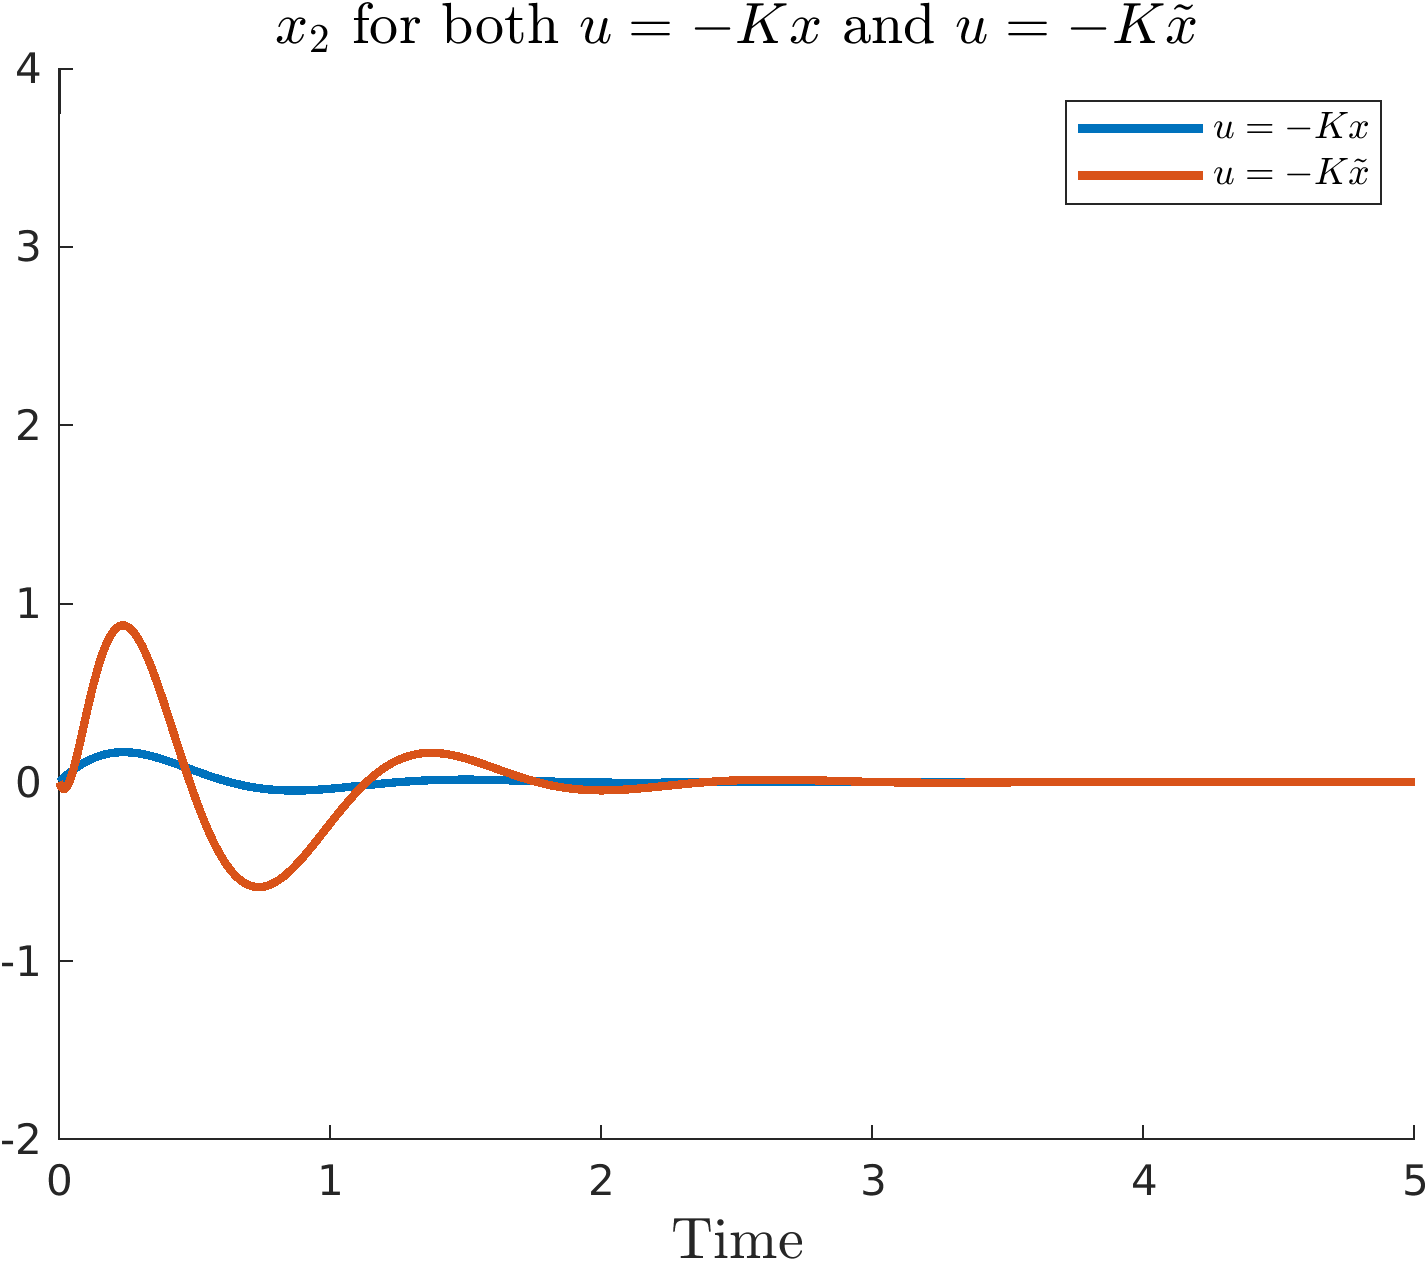
\includegraphics[width = \textwidth]{figures/c2-x2-plot.png}
    \end{subfigure}
    \caption{$x_1$ and $x_2$ for both $u = -\boldsymbol{K}x$ and $u = -\boldsymbol{K}\tilde{x}$}
    \label{fig:c-1_results}
\end{figure}

Comparing these two values, we see the observed state $\tilde{x}$ system starts diverging immediately, but then quickly adjusts and stabilizes slightly slower than the real response of the system with $x$.

\subsection*{Part 3}

In this part, we are tasked with exploring different $\mu$ values for our equation, as opposed to the $\mu_1 = \mu_2 = -10$ we utilized above. Below, we observe all three suggested values within this assignment: $\mu = \{ -10, -1, -0.1\}$:

\begin{figure}[H]
    \centering
    \begin{subfigure}{0.325\textwidth}
        \centering
        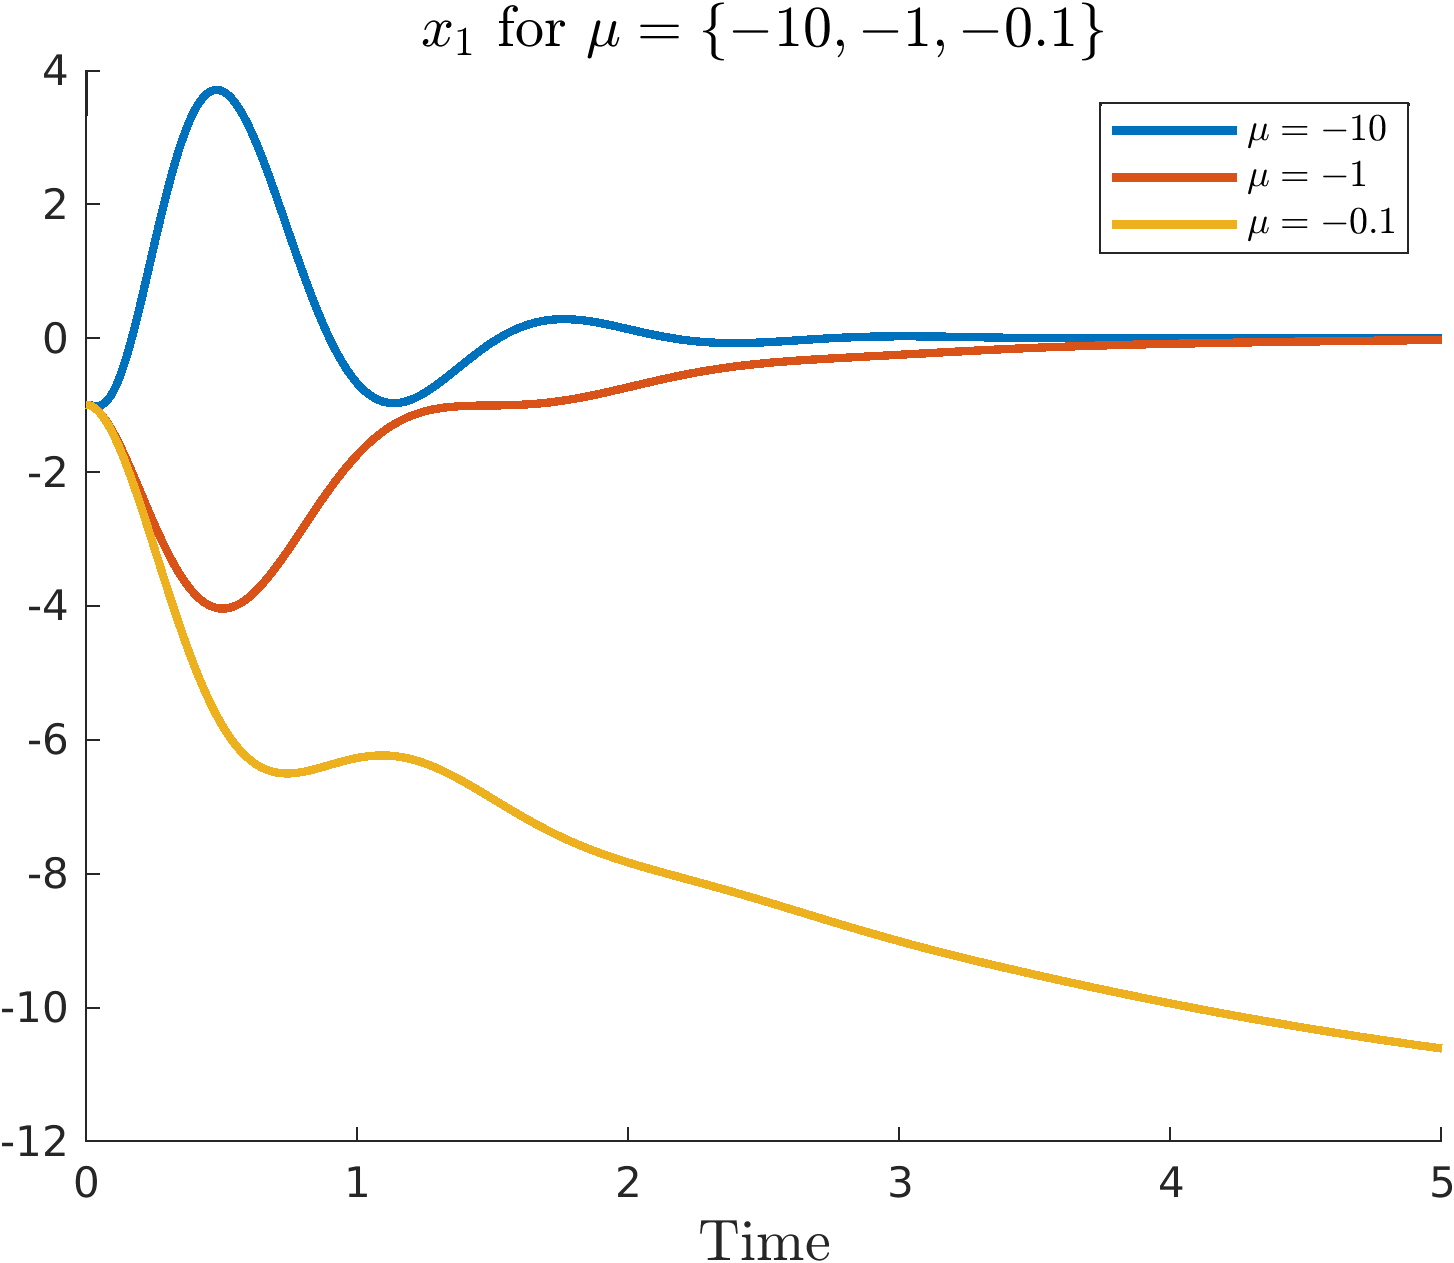
\includegraphics[width = \textwidth]{figures/c3-3-x1-plot.png}
        \caption{$x_1$}
    \end{subfigure}
    \begin{subfigure}{0.325\textwidth}
        \centering
        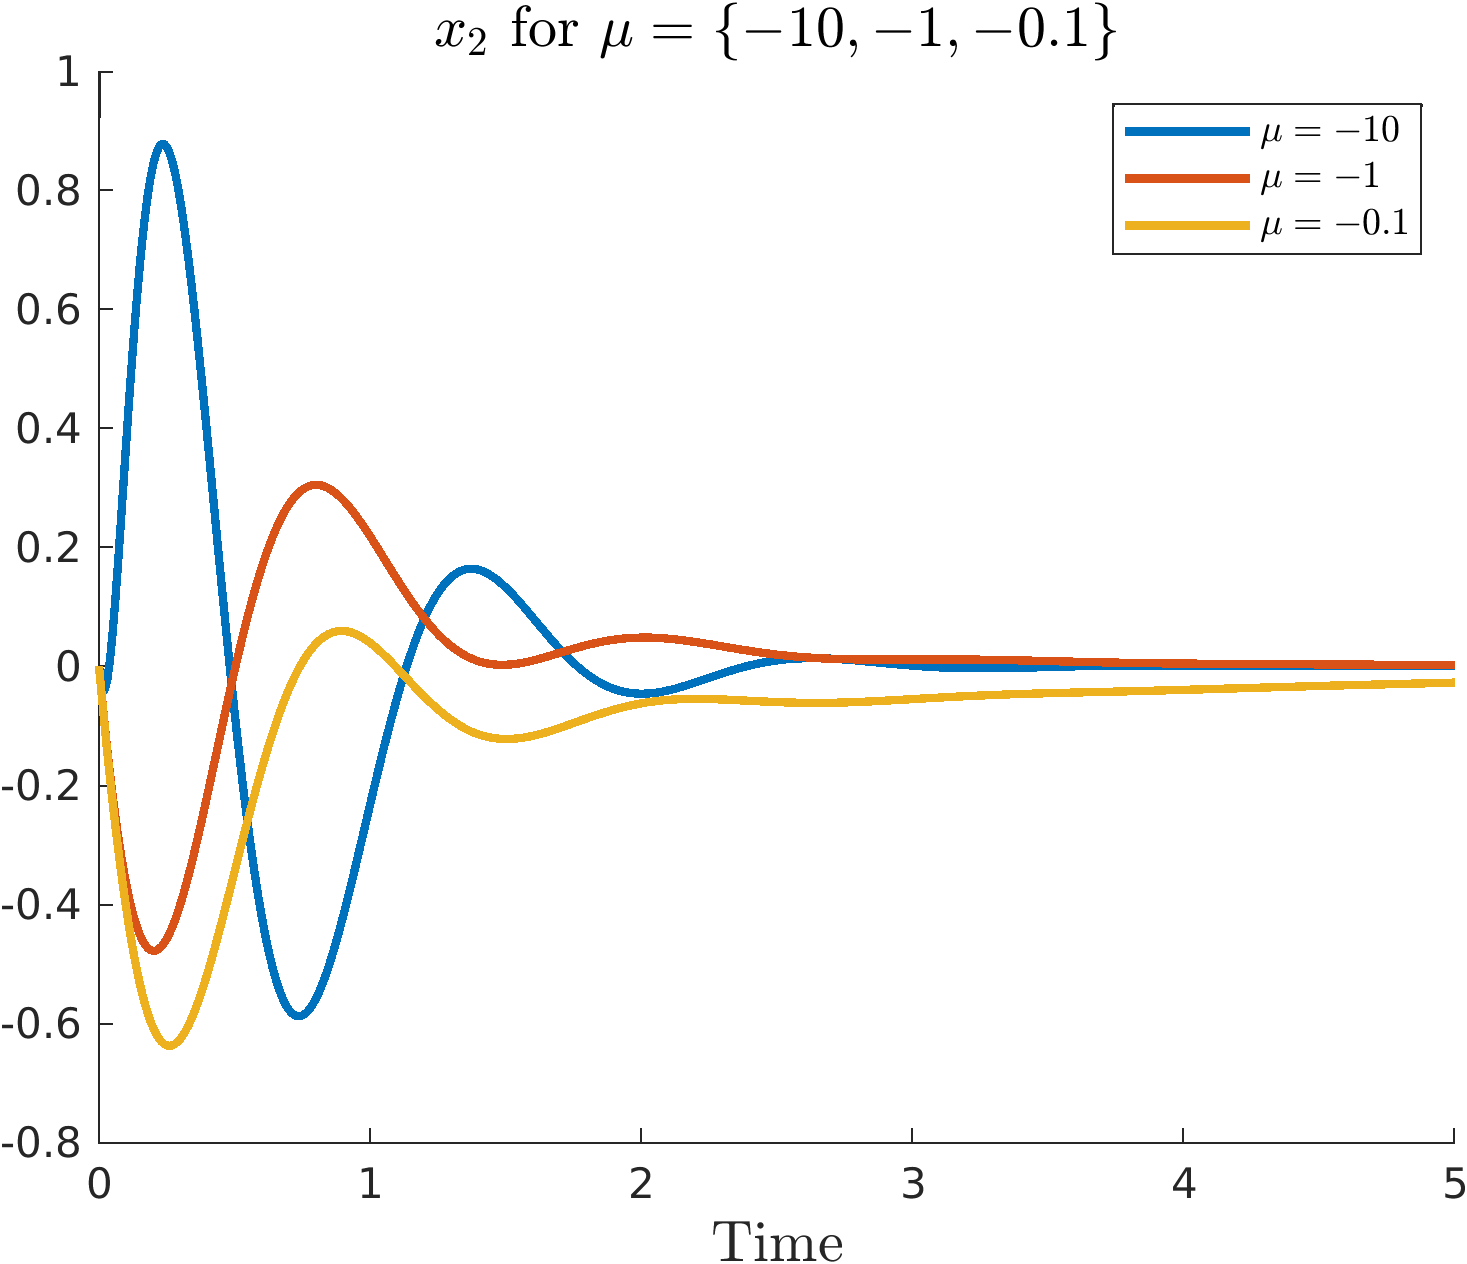
\includegraphics[width = \textwidth]{figures/c3-3-x2-plot.png}
        \caption{$x_2$}
    \end{subfigure}
    \caption{Observed response with different $\mu$ values}
    \label{fig:c-3_initial_look}
\end{figure}

Looking at these results, we can learn that choosing a $\mu$ affects the system in response time and magnitude of response. We see that the time for the observer-state feedback control syste to converge can be heavily delayed by selecting a $\mu$ too low, as we see with $\mu=-0.1$. The $x_1$ value for $\mu=-0.1$ looks as if it is diverging, but it is simply responding to the system extremely slowly. If we expand the range of time being observed, we see that it converges nearly 90 seconds later:

\begin{figure}[H]
    \centering
    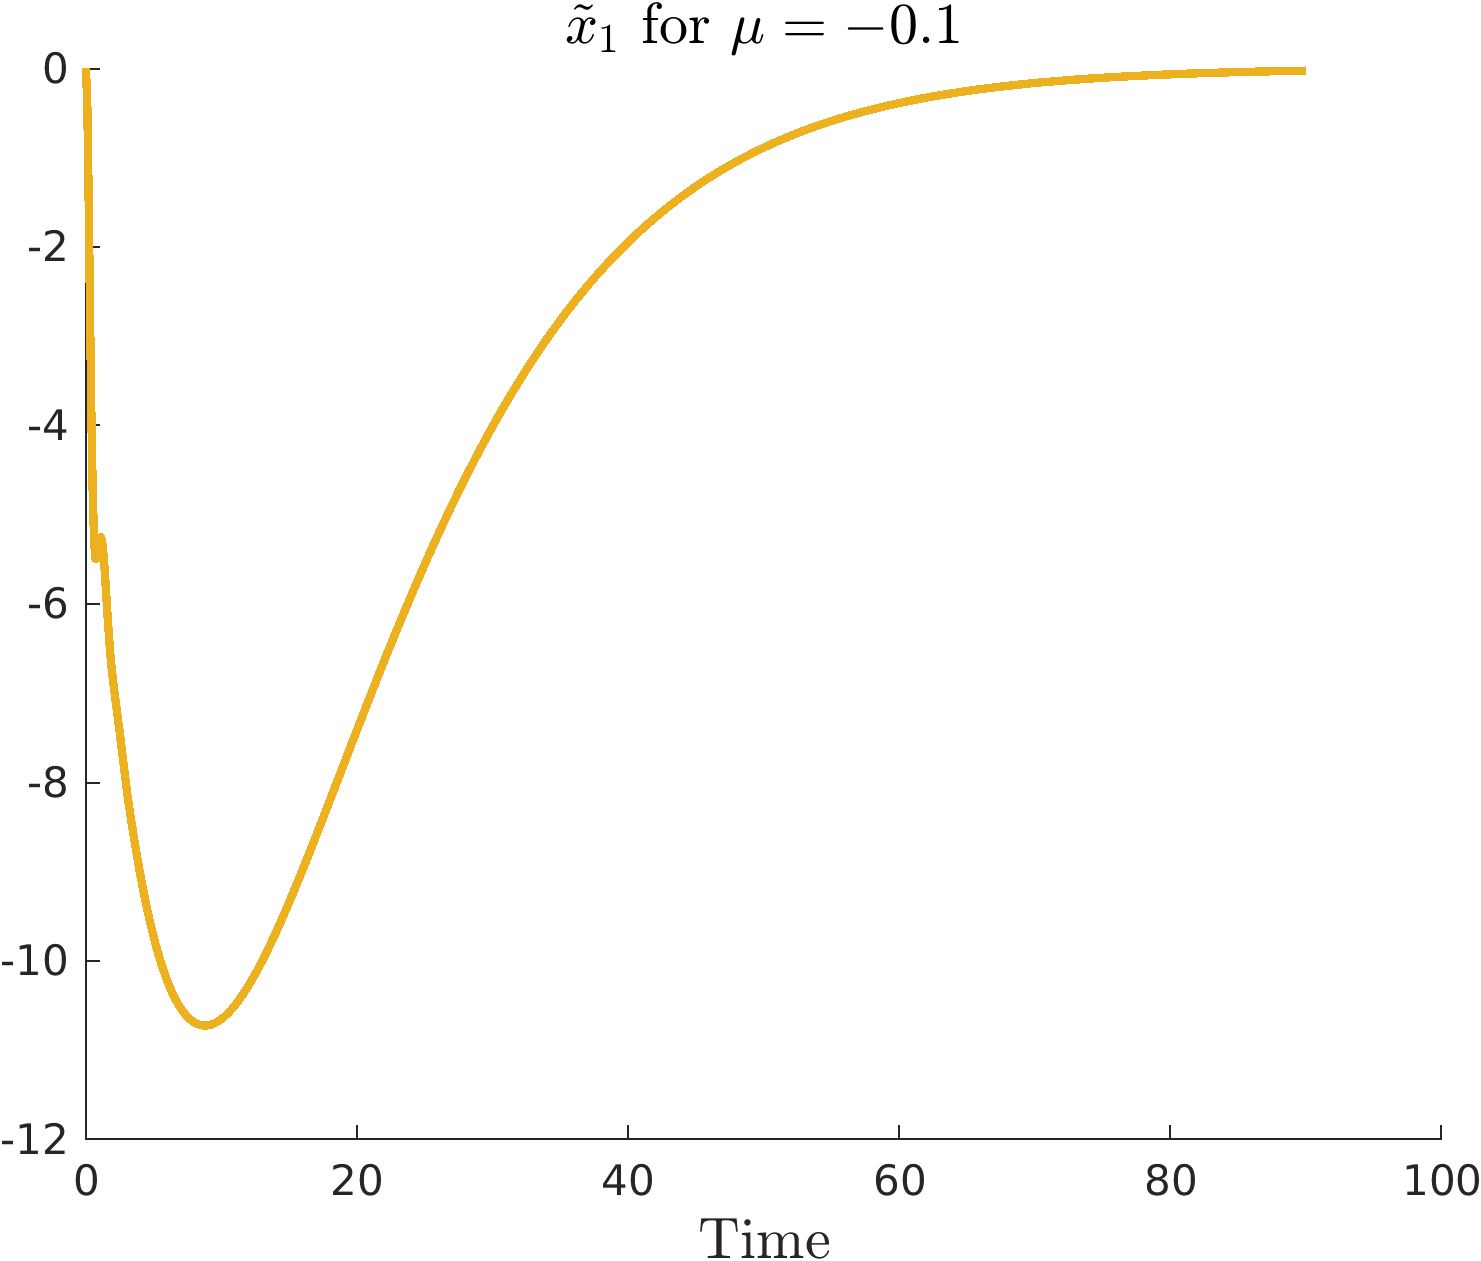
\includegraphics[width = 0.4\textwidth]{figures/c3-3-01-time-plot.png}
    \caption{$x_2$ convergence to $0$ with $\mu=-0.1$}
    \label{fig:mu_01_time}
\end{figure}

We also see from Figure $\refeq{fig:c-3_initial_look}$ that the $\mu$ results in the severity of the initial response of the system to a pertubation as well. compare $\mu=-1$ and $\mu=-10$. For $\mu=-1$ the initial response has a smaller magnitude, but ultimately converges slightly slower. This suggests that choosing a $\mu$ value allows one to tune both system response magnitude and time.

\subsection*{Part 4}

In this part, we are asked if the eigenvalues of the observed-state feedback system (ie $u = -\boldsymbol{K}\tilde{x}$) are the same as desired eigenvalues $\lambda_1 = -2+5i$ and $\lambda_2 = -2-5i$. If not, we are asked to to identify the eigenvalues of our observed-state feedback system.

First, we need to find what the eigenvalues of the observed-state feedback system are. To do this, we find the eigenvalues of $A-\boldsymbol{K}_e C$.  If we look at the eigenvalues for each $K_e$ we've calculated through this assignment, for $\mu=\{-10, -1, -0.1\}$, we see the following:

\begin{equation}
    \mu = -10 \to \sigma(A-\boldsymbol{K_e}C) = -10
\end{equation}

\begin{equation}
    \mu = -1 \to \sigma(A-\boldsymbol{K_e}C) = -1
\end{equation}

\begin{equation}
    \mu = -0.1 \to \sigma(A-\boldsymbol{K_e}C) = -0.1
\end{equation}

Thus, we see that the chosen $\mu$ value that we calculate the resulting $K_e$ ends up being the eigenvalues for $A-\boldsymbol{K}_e C$. Earlier, in Part 3, we looked at the effects caused by adjusting the $\mu$ values for the response sensitivity to error and how they affect convergence. This matches how we saw eigenvalues for chosen $K$ values in earlier systems when working with directly with the real state of the system.

Thus, from this, we can state that the eigenvalues of $A-\boldsymbol{K_e}C$, our $\mu$'s, can be selected in a manner to ensure that $\tilde{x}(t)$ will converge to 0 if $A-\boldsymbol{K_e}C$ is a stable matrix. We can choose these eigenvalues to create a sufficiently fast response than should converge to its origin at an adequate speed.

\end{document}